
%%%%%%%%%%%%%%%%%%%%%%%%%%%%%%%%%%%%%%%%%%%%%%
\section{Installation}


%%%%%%%%%%%%%%%%%%%%%%
\subsection{Anode Plane Assemblies (APAs)}

The APAs will be delivered to EHN1 in containers as shipped from the production sites.  These containers will be opened inside EHN1 and special lifting fixtures will be attached to each end of the APA.  The APA will be positioned and attached to two conveyances installed in EHN1.  Both conveyances will used to lift the APA from the container, oriented as shown in Figure~\ref{fig:apa-tooling} (right), and then rotate it 90$^\circ$ from that orientation, as in the left portion of the figure.
%the orientation from which it was shipped.  The lifting strap and fixtures will be removed for the lower edge of the APA. 
%This orientation of the APA is shown in Figure~\ref{fig:apa-tooling}.

\begin{cdrfigure}[The APA with the special tooling attached]{apa-tooling}{The APA with the lifting tooling attached.  The right image shows the orientation of the APA as delivered, the left shows the orientation when it is lowered into the material SAS. }
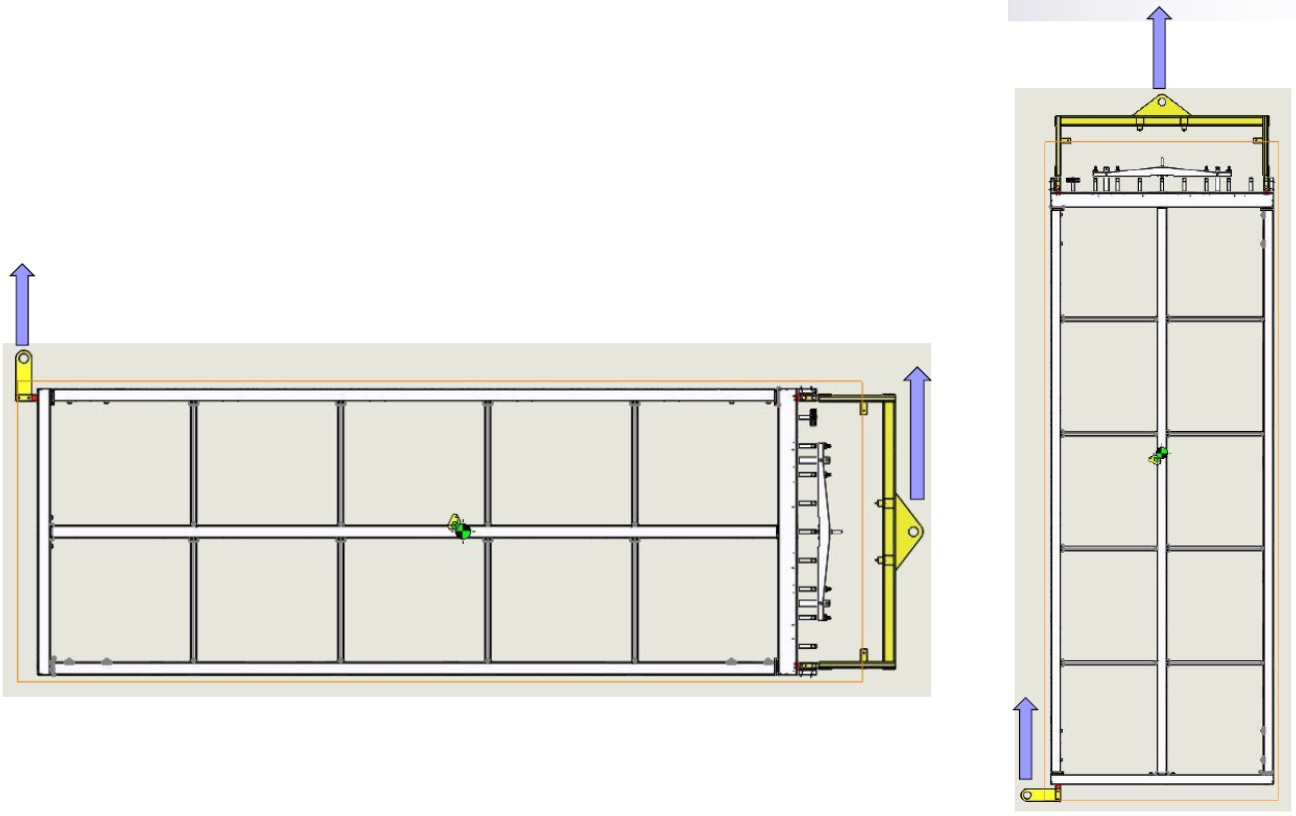
\includegraphics[width=0.7\linewidth]{apa-tooling}
\end{cdrfigure}

Once the APA is removed from the container and properly oriented, the lifting strap and fixtures will be removed for the lower edge of the APA, the roof hatch on the material SAS for 
\fixme{next to?} the clean room will be opened, and the APA will be lowered through the hatch.  The APA will then be transferred to a rolling trolley attached to a series of rails, and moved into the clean room via these rails.  These spaces and rails are described in more detail in Chapter~\ref{ch:spacereq}. 

Once in the clean room, the APA will go through a series of acceptance tests for both electrical integrity and wire tension.  It will also be inspected for broken wires or any other damage that could have resulted from shipment.  

%%%%%%%%%%%%%%%%%%%%%%
\subsection{Photon Detection System (PDS)}

After this testing is complete, the APA is integrated with the PDS.  There are ten PDs per APA, inserted into alternating sides of the APA frame, %.  This insertion alternates from one side to the other, with 5 PD being inserted into the APA 
five from each direction.  This is shown in Figure~\ref{fig:pds-install}.  Once a PD is inserted, it is attached mechanically to the APA frame with fasteners, a single electronics cable is attached, and strain is relieved.  Each PD is tested immediately after installation to ensure proper operation and to verify the cable readout.  

\begin{cdrfigure}[PDS installation]{pds-install}{PDS installation}
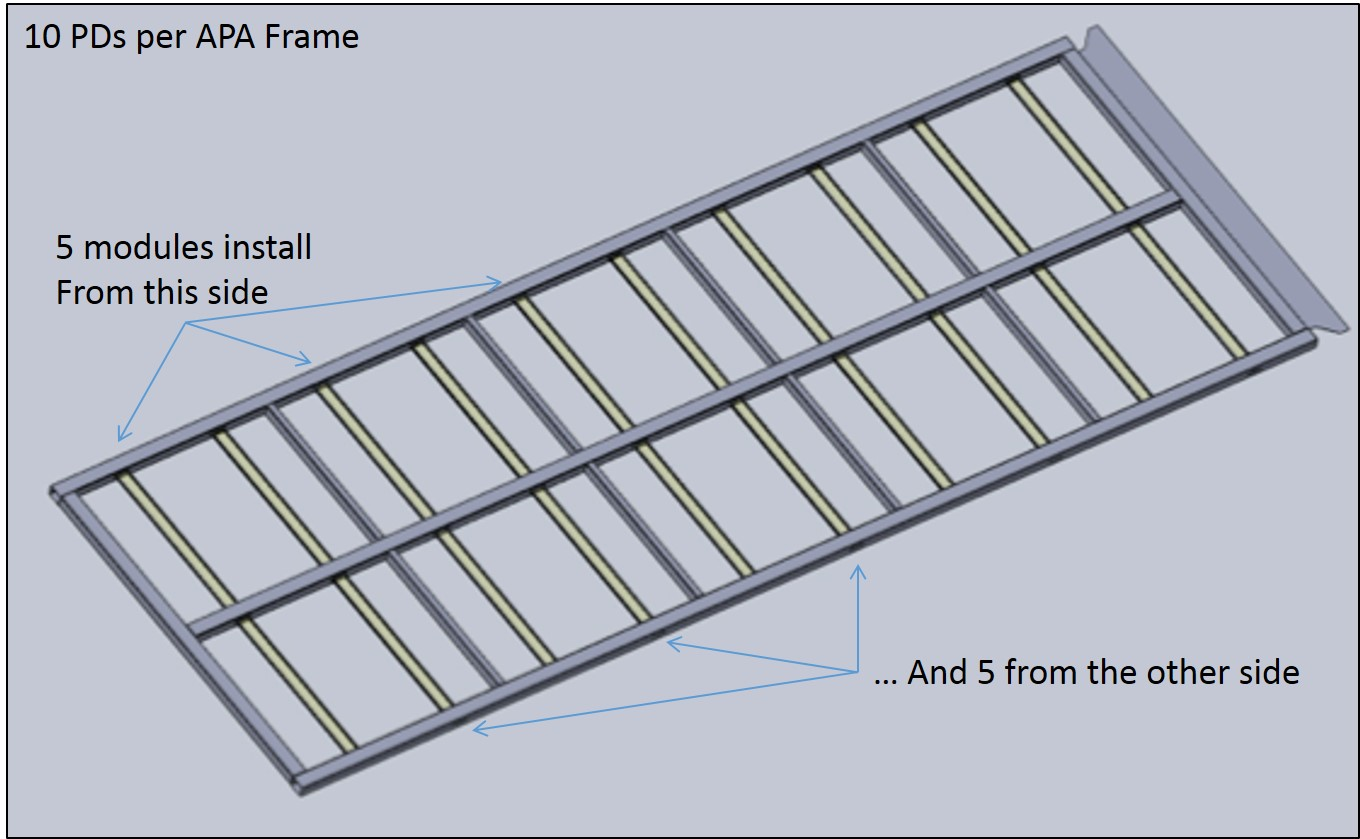
\includegraphics[width=0.7\linewidth]{pds-installation}
\end{cdrfigure}

%%%%%%%%%%%%%%%%%%%%%%
\subsection{Cold Electronics (CE)}
\label{subsec:ce_install}

Once the PD installation is complete 20 CE units are installed at the top of the APA frame.  Each CE unit consists of an electronics enclosure that contains the TPC read-out electronics inside.  Each unit also includes a bundle of cables that connect the electronics to the outside of the cryostat via the flange on the feedthrough port.  %Because access to the CE is not possible after the cryostat is sealed, a full complement of tests will be performed during the development stage and before the final installation -- move to QA
The location of the CE units on the APA is shown in Figure~\ref{fig:ce-install}.  These units will be connected via matching electrical connectors on the FEMB and the CR board mounted on the APA.  There will also be mechanical fasteners to hold the enclosure to brackets supported by the APA frame.  %Each of the CE units will be tested once installed to check connectivity.  

\begin{cdrfigure}[CE installation]{ce-install}{CE installation}
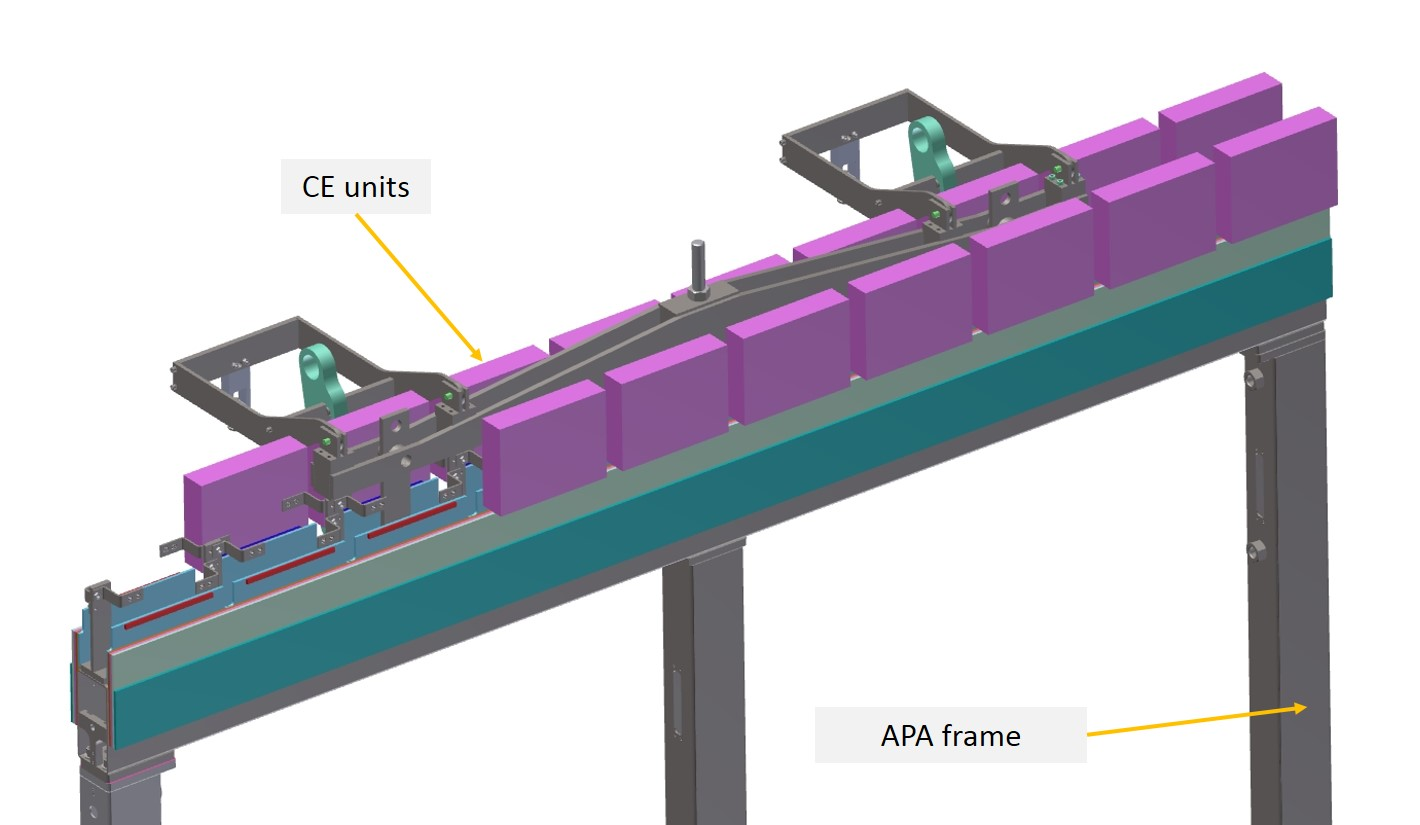
\includegraphics[width=0.7\linewidth]{ce-installation}
\end{cdrfigure}

After the APA has been fully integrated with the PDS and CE, it will be moved via the rails in the clean room to the integrated cold test stand.  This test stand, shown in Figure~\ref{fig:cold-test-stand-open}, is a large insulated box that is light-tight for PD testing and has a Faraday shield for CE testing.  At the top of the box is a crossing tube, similar to those in the cryostat, with a conflat fitting that accepts the warm-cold interface flange for the PD and CE cable connections.  To prepare for the series of warm electronics tests, the PD and CE cables will be routed and connected to their flanges, the APA will be moved inside the box, and the end cover that completes the Faraday cage will be installed.  %The warm tests are described in   \fixme{XXsectionXX}

Cold tests will follow the warm tests. Once the warm tests are complete, the inner volume of the enclosure will be purged with dry gas to reduce the moisture inside.  After this gas purge, the volume will be slowly cooled, using nitrogen gas, to a temperature of approximately 100 $^\circ$K.  The rate of cooldown must remain be less than 10 $^\circ$K/hr, the same as for cryostat cooldown.  The cooldown system is designed to maintain the inner volume near 100 $^\circ$K for approximately 48 hours.  The cold testing can take place during any of the three phases, i.e, during the cooldown period, the 48 hr ``cold'' period, or during the warmup.  After the cold testing is complete and the box has been purged of nitrogen with room air, it will be opened, the APA removed and he cables disconnected and secured for movement on the rail system.   
\fixme{why the cold testing can be done during cooldown or warm up could use some explanation. Why do you need to get down to 100 degrees when a warmer temperature would suffice, for example? Anne}

\begin{cdrfigure}[Cold test stand]{cold-test-stand-open}{A model of the integrated cold test stand in the ProtoDUNE-SP clean room in EHN1.}
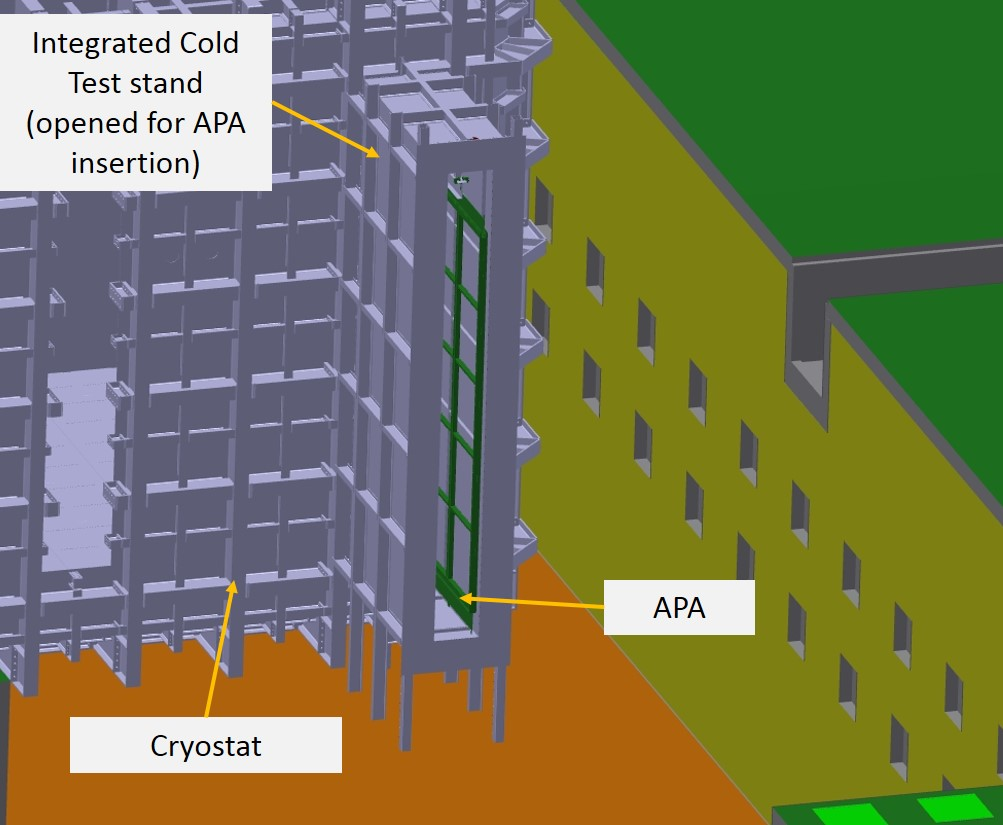
\includegraphics[width=0.7\linewidth]{cold-test-stand-open}
\end{cdrfigure}

Once cold testing is complete, the APA is ready to be moved into the cryostat via the rail system in the clean room.  The APA is moved through the TCO and transferred onto the appropriate rail in the detector support system.  Inside the cryostat, three APAs are needed to complete one row for the TPC.  %When the next two APAs are delivered, integrated and tested, 
As each of a set of three APAs completes testing, it is moved onto the same rail as its predecessors.  When all three are in place, the mechanical linkages between them are installed and the set is surveyed and locked into position. % in the beam direction.  Once positioned, the entire rail with the three APAs is translated in into position in the Y direction.  
%--- Anne thinks the above just adds unnecessary confusion.
The cables from each of the CE and PDs on the APA are then routed and connected to the final flanges on the cryostat.  After the first set of APAs is in place, the second set goes through the same testing and installation procedure.

%At the appropriate time in the installation sequence, the second trio of APAs will be moved into the cryostat and onto their detector support rail.  They will be surveyed and positioned in the same manner.


%%%%%%%%%%%%%%%%%%%%%%
\subsection{Cathode Plane Assemblies (CPAs)}

%\subsection{Assembly  and Installation }

%\fixme{Jack will revise this} 

Individual CPA modules will be delivered to EHN1 in containers as shipped from the production sites.  Each CPA module weights roughly 24~kg and will be lifted out of the shipping crate by hand. % and will not require and special fixtures. 
%
%Individual CPA panels will be assembled off site and shipped to CERN in the horizontal position.  Each panel weights roughly 24 kgs and therefore can be lifted out of the shipping crate by hand and will not require and special fixtures.
%
To construct each CPA, three CPA modules
will be placed on a flat surface and screwed/pinned together.  
\fixme{Do they come down to the SAS and into the clean room first, like the APAs? The FC does, so the CPAs must too, but it's not stated} 
  The crane \fixme{inside the cryostat?} then will be attached at the top end of the CPA with appropriate lifing straps and shackles.  The assembled CPA panel will be lifted to the vertical position.  

The load transfer from the crane hook to the installation rail still needs to be determined.  

Once two CPAs %planes 
are mounted they must be brought together within 1~mm along their (vertical) length.  (see thermal discussion in \fixme{Section 7}).  Two pins located on the side of the first CPA will fit into a vertical slot on the side of the second CPA to lock them together in the plane.  

The CPA %plane may
will not hang vertically %after being hung 
if the strap is not perfectly centered. %on center.  
This can be corrected when the FC is mounted to a pair of CPAs % planes.  
since the connection points on the FC are fixed and will therefore %tie the CPAs together and 
force the CPAs %them 
to hang vertically %because the assembly of the CPA planes and FC then becomes 
as together they become a two-point support structure.  

\fixme{I vote to remove the following sentence. Anne}
During assembly the FC will be hung from the CPA.  In a worst case scenario, the two FCs will be mounted on one side of the CPA first which will cause the CPA to rotate 2.9'' due to the offset loading.  



%%%%%%%%%%%%%%%%%%%%%%
\subsection{Field Cage (FC)}

%\subsection{Assembly Sequence and QC Procedures}

Three basic elements comprise the FC: the top, bottom and end-wall FC assemblies.  The top and bottom FC assemblies are basically mirror assemblies that are hinged from the top and bottom of the CPAs. % modules.  
Figure~\ref{fig:fc-assy} (left) shows a top/bottom FC assembly.  The ground plane covers one side of the field shaping profiles.  The right-hand image in the figure shows a top and bottom FC attached only to one side of the CPA. % module.  
These will be attached to both sides for the ProtoDUNE-SP installation.  \fixme{I don't find this image very illuminating. And how do you have a top and bottom attached to one side? Anne}

\begin{cdrfigure}[Top/bottom FC assembly]{fc-assy}{Top/bottom FC assembly }
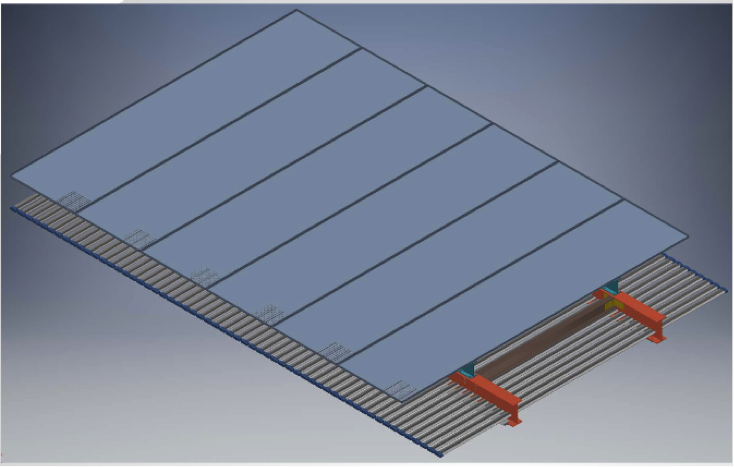
\includegraphics[width=.80\linewidth]{top-bottom-fc-assembly}
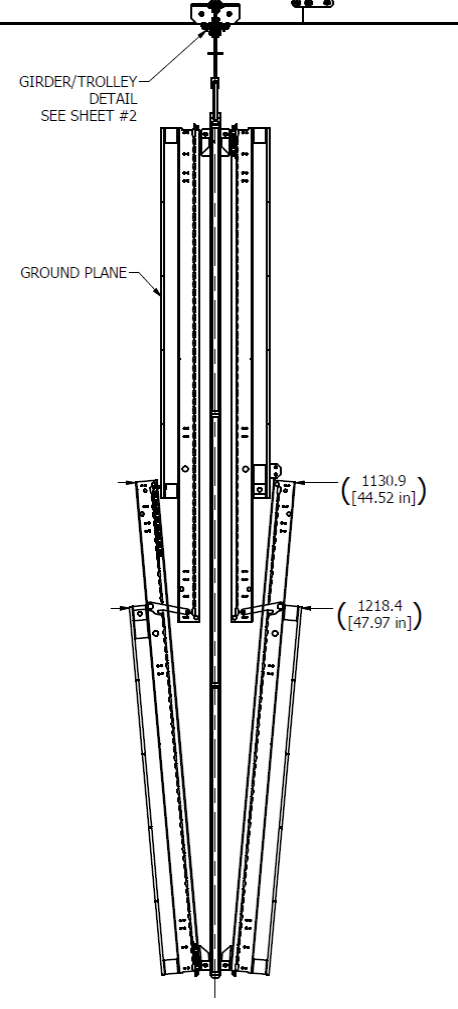
\includegraphics[width=0.1\linewidth]{fc-assy-vertical}
\end{cdrfigure}

The end-wall FC assembly is constructed from four stacked end-wall FC modules.  Figure~\ref{fig:fc-end-wall-panel} shows one of the end-wall FC modules.  %Four of these modules will be stacked and connected together to build the end-wall.  
The stacking will be done by the overhead hoist near the TCO in the clean room.  Once the end wall is complete, it will be moved into the cryostat on the rails in the clean room and positioned on the appropriate beam in the DSS. \fixme{Do we need to mention DSS for the APAs or CPAs?}  The end-wall is supported by a spreader bar that is in turn supported from the beam. The spreader can swivel about the support point;  this is necessary for positioning the end-wall with respect to the APA and CPA. % in the installation process.  

\begin{cdrfigure}[FC end wall panel]{fc-end-wall-panel}{FC end wall panel }
%\includegraphics[width=.80\linewidth]{}
\end{cdrfigure}
\fixme{Jack needs to remake the fc end wall panel picture}

The sequence of installation for the FC components is as follows:
\begin{itemize}
\item After the first row of APAs is installed and translated to the Sal\`{e}ve side of the cryostat, the two end-walls for the Sal\`{e}ve drift will be constructed and moved inside the cryostat supported 
by X beam B.  \fixme{shown in some figure?}
\item As the CPAs % modules 
are constructed outside the cryostat, both the top and bottom FC assemblies are attached on both sides, top and bottom.  This combination of FC and CPA is then moved into the cryostat and supported by X beam C.   \fixme{shown in some figure?}
This is done three times to get all into postion.
\item After the second row of APAs is installed and translated to the Jura side of the cryostat, the two end-walls for the Jura drift are constructed and moved inside the cryostat supported by X beam D.   \fixme{again, figure?}
\end{itemize}



